%parent:def:heegaardSplitting
%author:JeffHicks
%name:"Heegaard splitting for $S^3$"
%type:"figure"
%indepth:art:heegaardDiagram
%label:"fig:heegaardSplitting"
%parent:"exm:heegaardSplitting"
%caption:"After identifying $S^3\setminus \{(1, 0, 0, 0)\}$ with $\RR^3$ via stereographic projection, the Heegaard splitting of $S^3$ is given by taking the unit sphere, which decomposes the sphere into two $3$-balls. We also draw the meridinal line $(\cos(\theta), \sin(\theta), 0, 0)$."



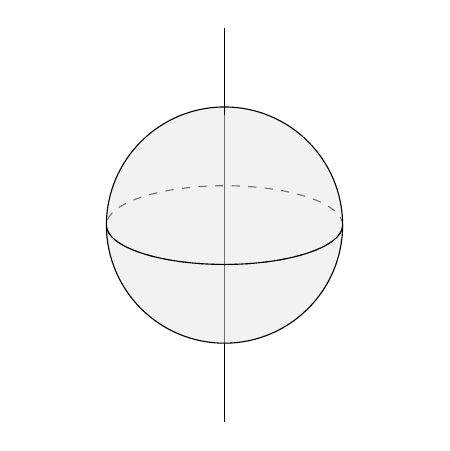
\begin{tikzpicture}
    \draw (-0.5,2) -- (-0.5,-3);
    \draw[dashed]  (-0.5,-0.5) ellipse (1.5 and 0.5);
    \draw[fill=gray!20, fill opacity=.5]  (-0.5,-0.5) ellipse (1.5 and 1.5);
    
    \draw (-0.5,2) -- (-0.5,0.9);
    
    \clip  (2,-0.5) rectangle (-3,-1.5);
    \draw  (-0.5,-0.5) ellipse (1.5 and 0.5);
    \end{tikzpicture}